\documentclass{physics_notes}

\title{Quantum Mechanics 2}
\author{St Aidan's Physics Society}
\date{\today}

\usepackage{physics}

\begin{document}

\maketitle
\begin{figure*}[h!]
	\centering
	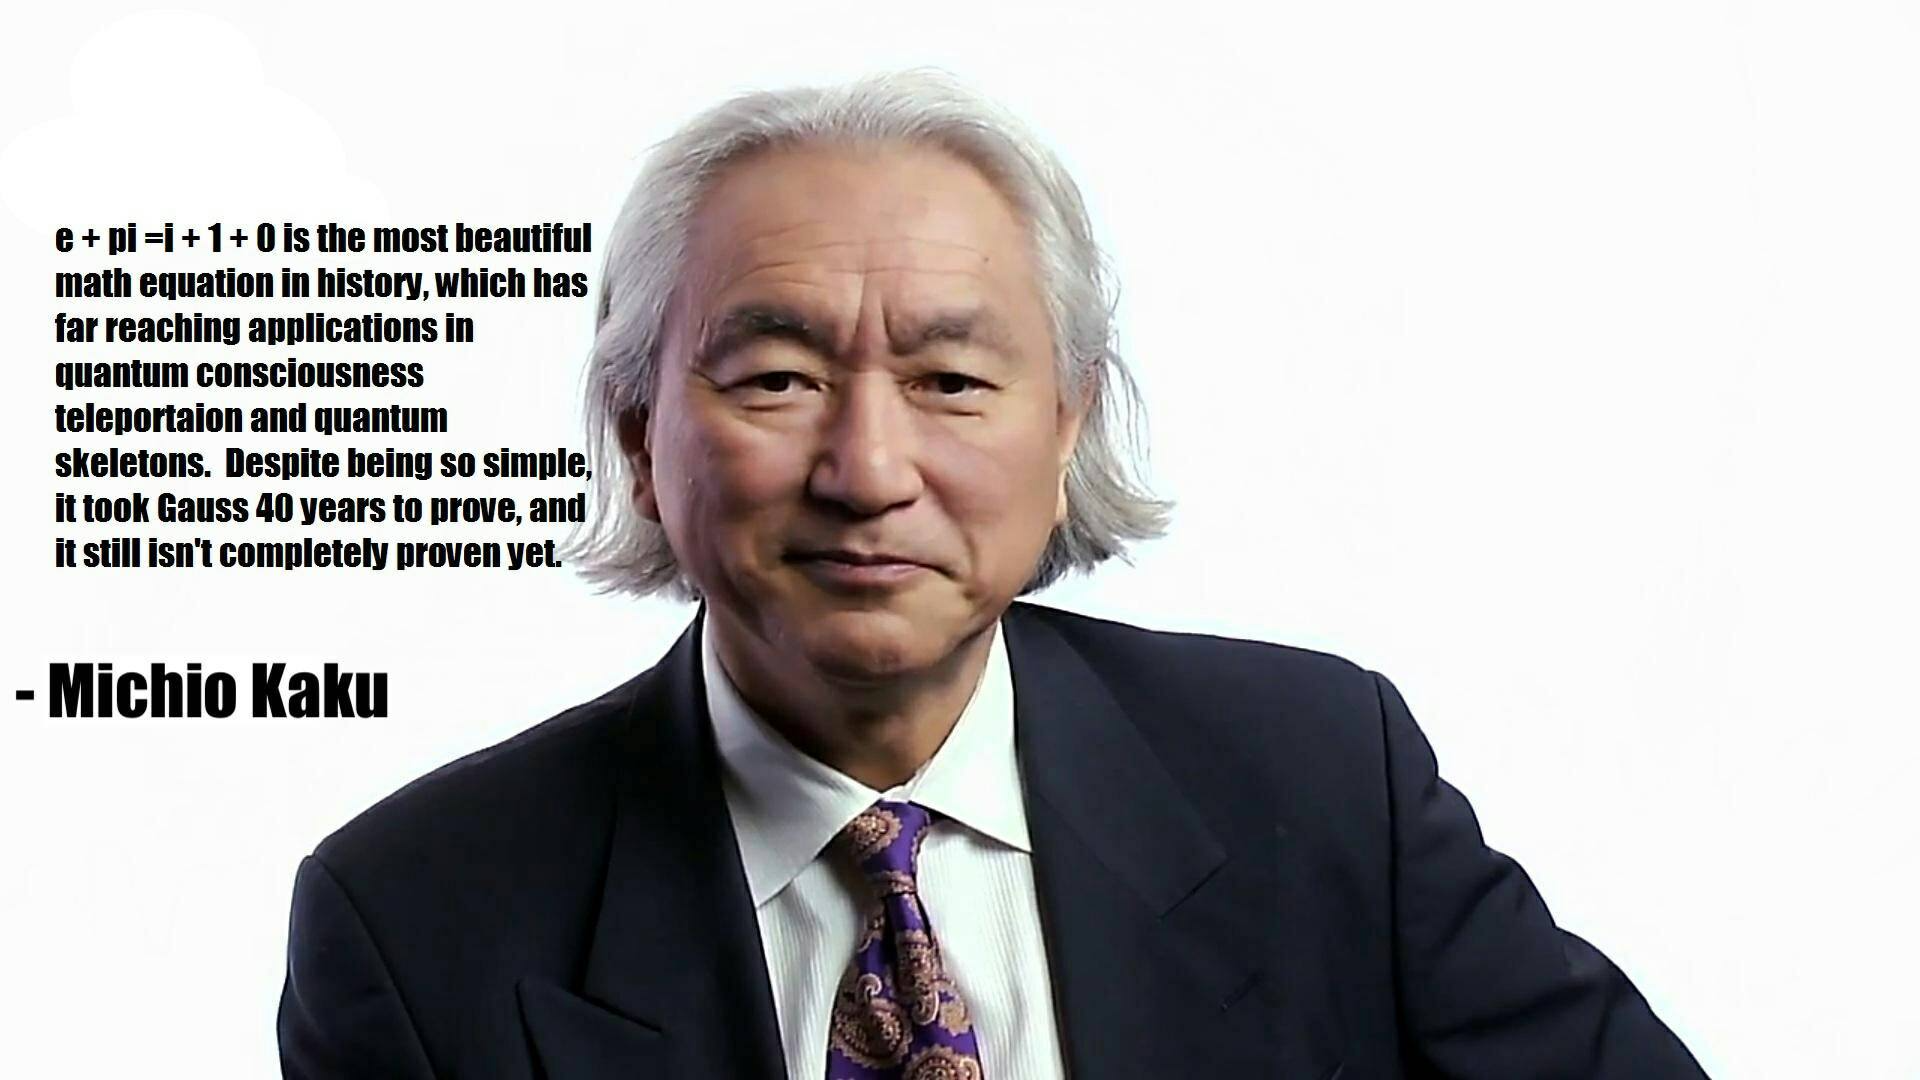
\includegraphics[width=\linewidth]{Figures/mich.png}
\end{figure*}
\tableofcontents
\newpage

\section*{Introduction}

These notes are designed to summarise the Foundations of Physics 2A (PHYS2581) Quantum Mechanics course, as taught by Prof. S Cole in the 2018/19 academic year. 

\section*{Summary}

\subsection*{The Five Postulates of Quantum Mechanics}

The content in this course can be summarised with the following five postulates:

\begin{enumerate}
	\item All possible predictions of the physical properties of a dynamical system can be obtained via its wavefunction.
	\item Every dynamical variable can be represented by a Hermitian operator, whose eigenvalues give the possible values of measurement of the dynamical variable. 
	\item The operators representing position and momentum are $x$ and $-i\hbar\nabla$ respectively. Operators for other dymanical variables can be derived using their corresponding dynaimcal variables' classical relations to position and momentum. 
	\item The probability of measuring a particular result of a superposition of states is given by the probability amplitude of the relevant eigenfunction, squared. 
	\item The time evolution of the wavefunction is described by the time-dependent Schr\"odinger equation.
\end{enumerate}

\section{Operators}\label{sec:operators}

All physical quantities in Quantum Mechanics can be represented by operators, which are essentially functions mapping from one space of physical states to another. From the $\hat{x} = x$ and $\hat{p} = -i\hbar\frac{\partial}{\partial x}$ operators along with time $t$, all other operators can be derived. For example, $\hat{E_k} = \frac{\hat{p}^2}{2m}$, as $E_k = \frac{p^2}{2m}$ classically. 

In quantum mechanics, these operators are made to act on wavefunctions (see §\ref{sec:wave_functions}): complex functions that describe everything we know about a system. The measureable values of the quantity represented by the general operator $\hat{Q}$ are the eigenvalues $q$ in the following eigenvalue problem:

\[ \hat{Q}\Psi = q\Psi \]

where $\Psi$ is the wavefunction of the system being measured. 

Classically, the Hamiltonian is usually the sum of kinetic and potential energies of a system. As such, we can define the Hamiltonian operator:

\begin{align*} 
\hat{H} &= \frac{\hat{p}^2}{2m} + V  \\
&= -\frac{\hbar^2}{2m} \frac{\partial^2}{\partial x^2} + V
\end{align*}

Using $\hat{H}{\Psi} = E\Psi$ (that the eigenvalues of the Hamiltonian are the allowed energy levels of the system), we obtain the Schr\"odinger equation. 


\subsection{Expectation}

The expectation of a general operator $\hat{Q}$ in 3D is given by:

\[ \expval{\hat{Q}} = \int_{V} \Psi^*\hat{Q}\Psi dV \]

The volume element $dV$ varies depending on the coordinate system. The volume element in some common 3D coordinate systems are given below. 

\begin{table}[h!]
\centering
	\begin{tabular}{c|c|c}
	Coordinate system & Position vector & Volume element \\ \hline
	Cartesian & $x\hat{\imath} + y\hat{\jmath} + z\hat{k}$ & $dxdydz$ \\
	Spherical polar & $r\sin{\theta}\cos{\phi}\hat{\imath} + r\sin{\theta}\sin{\phi}\hat{\jmath} + r\cos{\theta}\hat{k}$ & $r^2\sin{\theta}drd\theta d\phi$ \\
	Cylindrical polar & $\rho\cos{\theta}\hat{\imath} + \rho\sin{\theta}\hat{\jmath} + z\hat{k}$ & $\rho d\rho d\theta dz$
	\end{tabular}
	\caption{Volume element in common coordinate systems}
\end{table}
\subsection{Hermitian Operators}

If an operator $Q$ is Hermitian, then $Q^* = Q$. All operators that represent a real, measurable quantity are Hermitian as if $q$ is a measurable quantity, then we require that $q = q^*$, i.e. $q$ is real. So

\begin{align*}
\hat{Q}^*\Psi = q^*\Psi = q\Psi = \hat{Q}\Psi
\end{align*}

So $\hat{Q}^* = \hat{Q}$. Hence we see that if $q$ is measurable (and thus real), $\hat{Q}$ is Hermitian.


\subsection{Commutators}

The commutator of two operators $\hat{A}$, $\hat{B}$ is defined as $[\hat{A},\hat{B}] = \hat{A}\hat{B} - \hat{B}\hat{A}$. It follows that $[\hat{A},\hat{B}] = -[\hat{B},\hat{A}]$. If $[\hat{A},\hat{B}] =[\hat{B},\hat{A}] = 0$, then $\hat{A}$ and $\hat{B}$ are said to commute, meaning they share a common set of eigenfunctions.  Some important commutator identities are given below:

\begin{itemize}
	\item $[\hat{A},\hat{A}] = 0$
	\item $[\hat{A} + \hat{B}, \hat{C}] = [\hat{A},\hat{C}] + [\hat{B},\hat{C}]$
	\item $[\hat{A}\hat{B},\hat{C}] = \hat{A}[\hat{B},\hat{C}] + [\hat{A},\hat{C}]\hat{B}$
	\item $[\hat{A},\hat{B}\hat{C}] = [\hat{A},\hat{B}]\hat{C} + \hat{B}[\hat{A},\hat{C}]$
\end{itemize}

\subsection{Angular Momentum operators}

Two forms of angular momentum are important in quantum mechancics: orbital, and rotational. We will consider these separately, before looking at a more generalised approach.

\subsubsection*{Orbital Angular Momentum}

Orbital angular momentum is key for describing central potentials in 3D (e.g. the Hydrogen atom). Classically, orbital angular momentum, $\vec{L}$, is given by:

\begin{align*} \vec{L} = \vec{r} \times \vec{p} &= \begin{vmatrix} \hat{\imath} & \hat{\jmath} & \hat{k} \\ x & y & z \\ p_x & p_y & p_z \end{vmatrix} \\ &= (yp_z - zp_y)\hat{\imath} + (zp_x - xp_z)\hat{\jmath} + (xp_y - yp_x)\hat{k} \\ &= L_x \hat{\imath} + L_y \hat{\jmath} + L_z \hat{k} \end{align*}

with $L_x = (yp_z - zp_y)$, $L_y = (zp_x - xp_z)$, and $L_z = (xp_y - yp_x)$. Replacing position and mometum with their corresponding operators gives:

\begin{align*}
\hat{L_x} &= -i\hbar\left(y\frac{\partial}{\partial z} - z\frac{\partial}{\partial y}\right) \\
\hat{L_y} &= -i\hbar\left(z\frac{\partial}{\partial x} - x\frac{\partial}{\partial z}\right) \\
\hat{L_z} &= -i\hbar\left(x\frac{\partial}{\partial y} - y\frac{\partial}{\partial x}\right) 
\end{align*}

All three of these operators are Hermitian, and they do not commute with eachother. In fact, $[\hat{L_x}, \hat{L_y}] = i\hbar\hat{L_z}$, $[\hat{L_y}, \hat{L_z}] = i\hbar\hat{L_x}$, $[\hat{L_z}, \hat{L_x}] = i\hbar\hat{L_y}$. This non-commutation means we can only know the component of orbital angular momentum in one direction at any time, and gives rise to an uncertainty principle:

\[ \sigma_{\hat{L_x}}\sigma_{\hat{L_y}} \geq \frac{1}{2}\left|\expval{[\hat{L_x},\hat{L_y}]}\right| = \frac{\hbar}{2}\left|\expval{\hat{L_z}}\right| \]

However, we can obtain more information about the system by defining $\hat{L^2} = \hat{L_x^2} + \hat{L_y^2} + \hat{L_z^2}$ as we see $[\hat{L^2},\hat{L_x}] = [\hat{L^2}, \hat{L_y}] = [\hat{L^2}, \hat{L_z}] = 0$, and so we can know a component of orbital angular momentum and the total angular momentum simultaneously. 
\subsection{Ladder Operators}

\section{Wave functions}\label{sec:wave_functions}
\subsection{Probability distributions}
\subsection{Superposition}
\subsection{Eigenfunctions of various potentials}

\section{Relativistic corrections}\label{sec:relativistic_corrections}
\subsection{Non-degenerate perturbation theory}
\subsection{Degenerate perturbation theory}
\subsection{The Hydrogen atom}
\subsubsection{Degenerate perturbation theory in hydrogen}
\subsubsection{Hydrogen fine splitting}




\end{document}